\renewcommand{\encodingdefault}{OT1}
\documentclass[conference]{IEEEtran}
\IEEEoverridecommandlockouts
% The preceding line is only needed to identify funding in the first footnote. If that is unneeded, please comment it out.
\usepackage{cite}
\usepackage{amsmath,amssymb,amsfonts}
\usepackage{algorithmic}
\usepackage{graphicx}
\usepackage{textcomp}
\usepackage{xcolor}
\usepackage{hyperref}
\usepackage{minted}
\def\BibTeX{{\rm B\kern-.05em{\sc i\kern-.025em b}\kern-.08em
    T\kern-.1667em\lower.7ex\hbox{E}\kern-.125emX}}
\begin{document}

\title{Jitsi on OpenBSD\\
{\Large Puffy presents video conferencing}
}

\author{\IEEEauthorblockN{Philipp Buehler}
\IEEEauthorblockA{
\textit{sysfive.com GmbH}\\
Hamburg, Germany \\
pb-openbsd@sysfive.com}

}

\maketitle

\begin{abstract}
This paper will cover all bits and bolts to fully understand the components
at play, their intercommunications and how this knowledge can be used to create
a Jitsi-on-OpenBSD setup that features a restricted (compartmentalized) setup using
dedicated machines or -as shown- VMM based VMs, where each VM runs only one of the
components.

It'll be documented what's necessary to create a sensible pf.conf on each VM and how to
add reverse proxy (relayd, haproxy) for distribution of workload.

Also covering pitfalls/hints along underlying components and what to lookout for on 
the client/browser side for interopability.
\end{abstract}

\begin{IEEEkeywords}
Jitsi, OpenBSD, VMM
\end{IEEEkeywords}

% XXX
%\section{Examples}
%Just some template code
%\begin{minted}{c}
%int main(){
% printf("hello");
%}
%\end{minted}
%\subsection{Units}
%\begin{itemize}
%\item Use either SI (MKS) or CGS as primary units. (SI units are encouraged.) English units may be used as secondary units (in parentheses). An exception would be the use of English units as identifiers in trade, such as ``3.5-inch disk drive''.
%\item Use a zero before decimal points: ``0.25'', not ``.25''. Use ``cm\textsuperscript{3}'', not ``cc''.)
%\end{itemize}
% XXX

\section{Introduction}
Jitsi and OpenBSD are both not covered much as a documented setup. Installation documents
for Jitsi are almost always about Linux OS (and there mostly Debian) and do not cover
some internals. The reference documentation on the other hand can be very overwhelming.

There is some FreeBSD ``all in one'' port (package) with no explanation and it cannot be
used to install core components (only) on different nodes.

This documentation is to show a distributed install on OpenBSD using pre-packages and
need-to-function (minimum) firewall settings (`pf.conf`).

The described configurations will enable a fully integrated video conferencing
to be available at `https://jts.fips.de` - adapt the setting accordingly for your domain.

\section{Riddles}
Both major players show obstacles that have to be overcome to gain a functioning installation.
\subsection{Jitsi}
A "full blown" Jitsi installation can consist over over a dozen components and all the
necessary networking/firewalling configuration can be exhaustive. Any possible discovery
magic is not documented.

Some configuration snippets are undocumented and tend to make the understanding poorer
not better. Worst example are necessary DNS settings and `nginx.conf.`

The typical answer to be found on asking question is to use the official `all-in-one`
Debian VM.

\subsection{OpenBSD}
This also leds to the question if it's possible to run a (core) Jitsi installation on
OpenBSD only or if there's need be for Linux (VM).

Also it's a bit difficult to find example-based documentation on VMM, e.g. for using
VMM as the core router, too. (Combination `vm.conf`+`pf.conf`s).

Can we scale the installation horizontally and how to use Java based applications
with `rcctl`.
\section{Components}
\subsection{OpenBSD}
In this example setup I make heavy use of `VMM` eco system on OpenBSD which consists of:
\begin{itemize}
\item `vmm(4) - virtual machine monitor:`
    kernel driver isolating/providing the required resources for the VMs (“hypervisor”)
\item `vmd(8):`
	userland daemon to interact with `vmm`
\item `vmctl(8)`:
	administrative tool to create, start/stop, .. VMs
\item `vm.conf(5)`:
	persist VMs resource configuration
\end{itemize}
\subsection{Jitsi}
A `core` (basic video conferencing) setup comprised by:
\begin{itemize}
\item `nginx(8)` web:
	serving web assets and reverse proxy BOSH or websockets
\item `prosody(8)` xmpp:
	conference chat + internal components communication (esp. “PubSub” for health/discovery)
\item `jicofo` JItsi COnference FOcus:
	room+session handling in conferences (who’s talking to whom and where)
\item `jvb` videobridge:
	mediastream (WebRTC) handlings between participants (SFU)
\item `jibri` JItsi BRoadcasting Infrastructure (optional):
	recording + streaming conferences
\end{itemize}

\section{Architecture}
To host the Jitsi components in a VM each, this uses the following architecture (see Figure 1).
\begin{figure*}
    \centering
    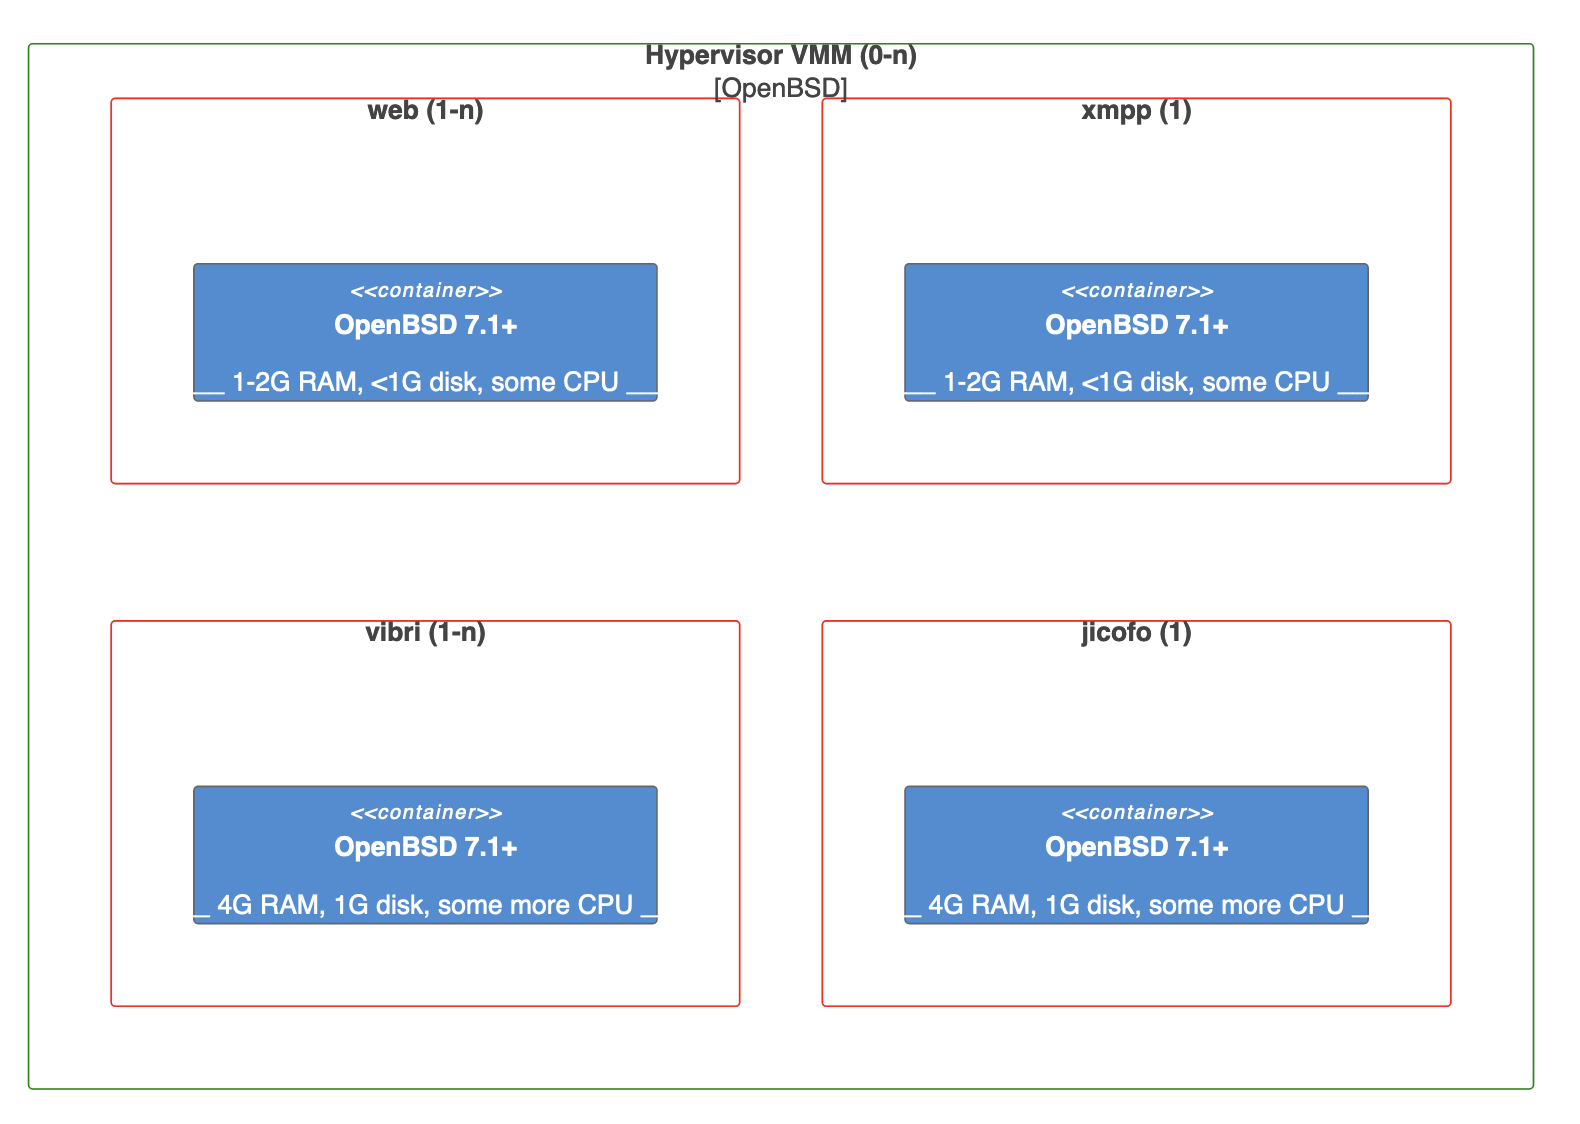
\includegraphics[width=16cm]{img/arch-openbsd.png}
    \caption{\textsf{OpenBSD VMM architecture}}
\end{figure*}
\section{Communications}
Communications between the components and the logical `publication` + `subscription` in Jitsi
is as follows (needed in `pf.conf` later on) (see Figure 2+3).
\begin{figure*}
    \centering
    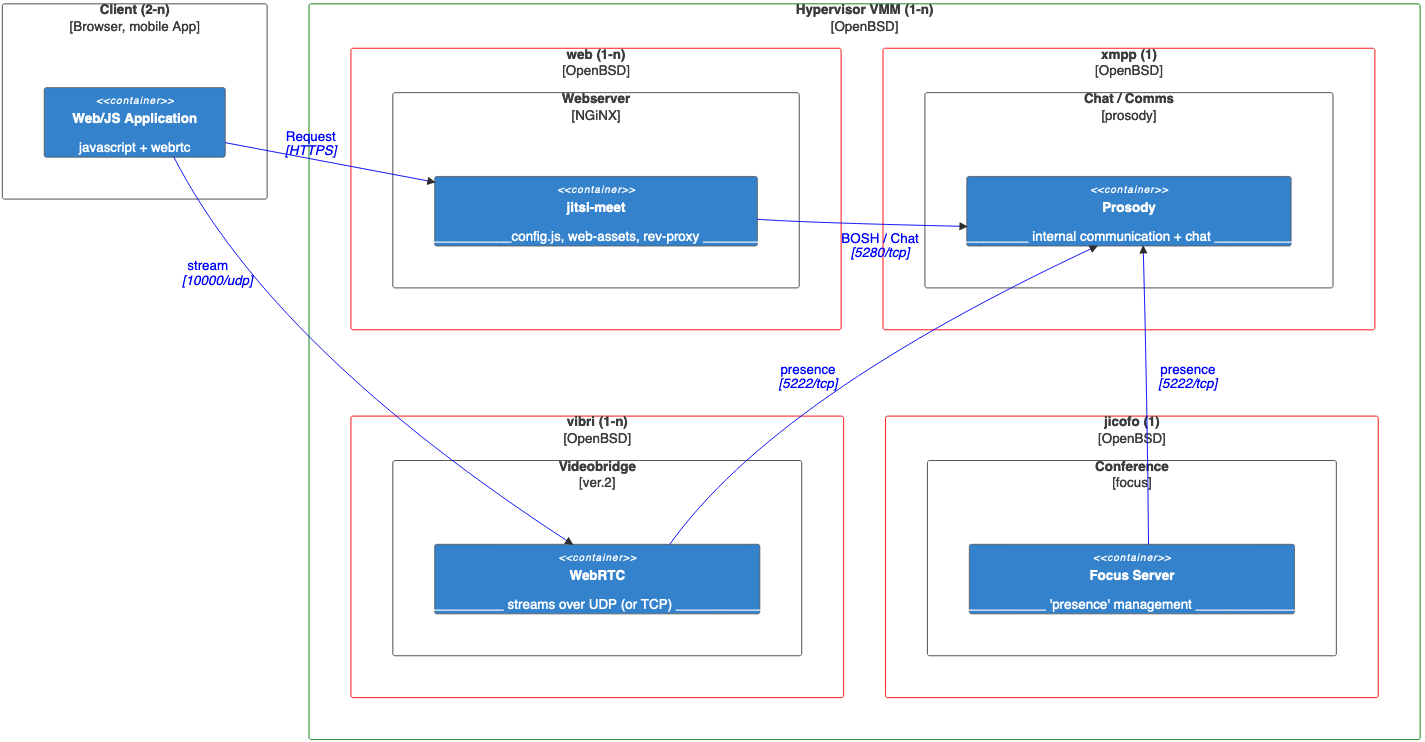
\includegraphics[width=16cm]{img/arch-tcp.png}
    \caption{\textsf{OpenBSD VMM architecture}}
\end{figure*}
\begin{figure*}
    \centering
    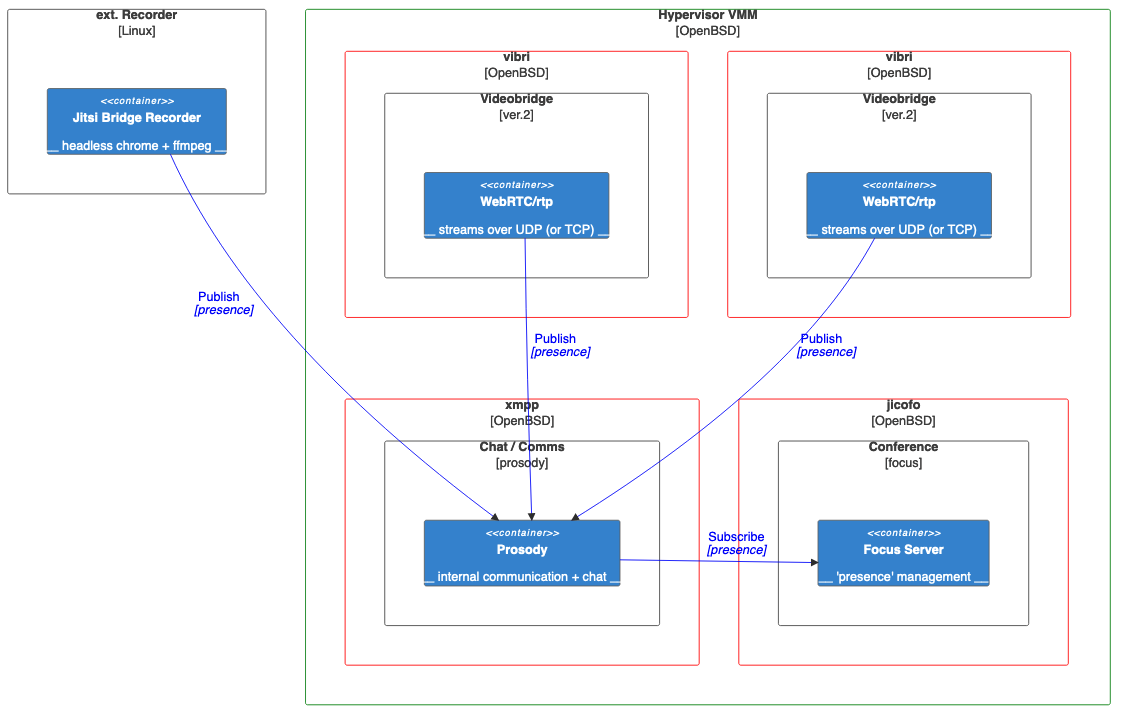
\includegraphics[width=16cm]{img/arch-pubsub.png}
    \caption{\textsf{OpenBSD VMM architecture}}
\end{figure*}

\section{Installation}
The installation is structered in the following steps:
\begin{itemize}
\item create VM images
\item construct /etc/vm.conf
\item add hosts / DNS
\item `nginx`: install, config, certs
\item `prosody`: pkg install, config, certs, users
\item `jicofo`: pkg install, config
\item `jvb`: pkg install, config
\end{itemize}
\subsection{VM setup}
To create an VM image being used in the following setup:
\begin{minted}{bash}
rcctl enable vmd; rcctl start vmd
mkdir /home/vmm; cd /home/vmm
vmctl create -s 5G web.qcow2
ftp https://cdn.openbsd.org/pub/OpenBSD
/7.1/amd64/install71.iso
vmctl start -m 2G -L -i 1 -r install71.iso\
-d /home/vmm/web.qcow2 web
vmctl console web
## run the (I)nstaller, default options.
## only one 'a' slice on (w)hole disk
## halt -p (so new sshd_keys per VM)
vmctl stop web
for vm in xmpp jicofo jvb ; do 
cp web.qcow2 \${vm}.qcow2; done
echo 'net.inet.ip.forwarding=1' >> \\
/etc/sysctl.conf
\end{minted}
The VM definitions in `/etc/vm.conf` as follows. The "instance" tells `vmctl`
to use "web"'s configuration as a template and only adapt changes like "disk"
or "memory" to it.
\begin{minted}{bash}
vm "web" {
  enable
  memory 2G
  disk "/home/vmm/web.qcow2" format qcow2
  local interface { up }
}
vm "web" instance "xmpp" {
  disk "/home/vmm/xmpp.qcow2" format qcow2
}
vm "web" instance "jicofo" {
  memory 4G
  disk "/home/vmm/jicofo.qcow2" format qcow2
}
vm "web" instance "jvb" {
  memory 4G
  disk "/home/vmm/jvb.qcow2" format qcow2
}
\end{minted}
\subsection{DNS + /etc/hosts}
DNS: ONE A-RR for jts.fips.de; but local hosts for jicofo (or split DNS).

The following `/etc/hosts` needs to be on each VM and on the VMM host.
Use these names in `/etc/myname`, too.
\begin{minted}{bash}
100.64.1.3    web
100.64.2.3    xmpp jts.fips.de
100.64.3.3    jicofo
100.64.4.3    jvb
\end{minted}
\section{Firewalling}
On each VM the following `pf.conf` is for good (admin) measure:
\begin{minted}{bash}
block return log
pass out quick on egress proto { tcp udp }
  to any port { 123 53 80 443 }
pass in quick on egress proto tcp 
  from \$admin to port 22
\end{minted}
\subsection{VMM}
Assumption that all traffic hits the VMM external IP-address (on egress) here:
\begin{minted}{bash}
pass in on egress proto tcp to any 
  port { 80 443 } rdr-to web
pass in on egress proto udp to any 
  port { 10000 } rdr-to jvb
pass in proto tcp from { jvb jicofo } 
  to xmpp port 5222 # native
pass in proto tcp from web to xmpp 
  port 5280 # http/BOSH
pass in on egress proto tcp to any 
  port 5280 rdr-to xmpp # debug
# DNS
vms={ web xmpp jicofo jvb }
pass in proto { udp tcp } from \$vms 
  to any port domain rdr-to \$resolver
\end{minted}
\subsection{web/nginx}
The webserver needs the basic ports and for the proxy connection to BOSH an outgoing to 5280/tcp.
\begin{minted}{bash}
pass in quick on egress proto tcp
  to self port { 80 443 }
pass out quick on egress proto tcp
  to xmpp port 5280
\end{minted}
\subsection{prosody}
The XMPP "native" only used from jicofo and jvb. The BOSH as above and if need be
the dedicated auth via 5347/tcp (not covered here).
\begin{minted}{bash}
pass in proto tcp from { jicofo jvb }
  to self port { 5222 }
pass in proto tcp from web
  to self port 5280
pass in proto tcp from { \$admin }
  to self port { 5280 5347} # debug
\end{minted}
\subsection{jicofo}
Jicofo talks to prosody as above. The webclient connects to jicofo via 10000/udp. There
is an administrative connection possible to 8080/tcp to establish e.g. monitoring with prometheus.
for scale out the 10000/udp can be changed and would make use of a port range e.g. 
‘10000:10050’ vertically or explicit rdr-to in VMM for horizontally.

\begin{minted}{bash}
pass out quick on egress proto 
  tcp to xmpp port { 5222 5280 }
pass in quick on egress proto 
  udp to self port 10000
pass in quick on egress proto 
  tcp from \$monitor to self port 8080
\end{minted}
\subsection{videobridge}
The videobridge only needs to reach out to prosody. The monitoring exporter on 8888/tcp
seems to be broken (no values) as of this writing.
\begin{minted}{bash}
pass out quick on egress proto
  tcp to xmpp port 5222
pass in quick on egress proto
  tcp from \$monitor to self port 8888
\end{minted}

\section{Prosody}
To install prosody some simple steps are enough:
\begin{minted}{bash}
pkg_add unzip-- prosody
prosodyctl install \
 --server=https://modules.prosody.im/rocks/ \
 mod_client_proxy
prosodyctl install \
 --server=https://modules.prosody.im/rocks/ \
mod_roster_command
\end{minted}
The modules do not need further configuration in `prosody.cfg.lua`.
`client\_proxy` gets loaded with "Component" configuration. `roster\_command` is CLI only.
The configuration key bits in `/etc/prosody/prosody.cfg.lua` are:
\begin{minted}{bash}
http_interfaces = { "*", "::" }
VirtualHost "jts.fips.de"
    authentication = "anonymous";

    modules_enabled = { "bosh";
      "pubsub"; }
    c2s_require_encryption = false

VirtualHost "auth.jts.fips.de"
    admins = { "focus@auth.jts.fips.de",
     "jvb@auth.jts.fips.de" }

    ssl = { key =
     "/var/prosody/auth.jts.fips.de.key";
        certificate =
    "/var/prosody/auth.jts.fips.de.crt"; }

    authentication = "internal_hashed"
    
Component "conference.jts.fips.de" "muc"
Component "jvb.jts.fips.de"
    component_secret = "CHANGE_jvb"
Component "focus.jts.fips.de" "client_proxy"
    target_address = 
      "focus@auth.jts.fips.de"
Component "internal.auth.jts.fips.de" "muc"
    muc_room_locking = false
    muc_room_default_public_jids = true
\end{minted}
The additional `FQDN` are internally only and
do NOT need any DNS configuration (like an
HTTP `Host` header).

It's possible that `jvb` follows the example of
`focus` to change authentication from shared secret
to a user (`target\_address`).
\subsection{Users}
The connection for `jvb` uses a shared secret as shown on the previous page.
For further users in use here:
\begin{minted}{bash}
rcctl enable prosody
rcctl start prosody
prosodyctl register focus \
  auth.jts.fips.de CHANGE_FOCUS
prosodyctl mod_roster_command \ 
  subscribe focus.jts.fips.de \
  focus@auth.jts.fips.de
\end{minted}
\subsection{TLS}
Besides WebRTC demanding to use `https` between browser and server side, we shall
encrypt all internal traffic, too. For the prosody connections:
\begin{minted}{bash}
prosodyctl cert generate \
  auth.jts.fips.de
# fill in `openssl req` dialog

cd /var/prosody
yes | /usr/local/jdk-11/bin/keytool
  -import -alias prosody -file \
  auth.jts.fips.de.crt -keystore \
  jicofo-key.store -storepass jitsicool
  
cp jicofo-key.store jvb-key.store 
# copy to VM jicofo and jvb accordingly
\end{minted}
`keytool` comes with JDK, this task can also be done on jicofo or jvb VM - or copy
over the resulting store-files to jicofo/jvb VM respectivly.
Do NOT change JDK's `lib/security/cacerts` - any later upgrade from jdk-11
would "forget" the changed keystore.

\section{nginx}
To install nginx and the jitsi web elements (javascript, images, ..) only two packages
are needed:
\begin{minted}{bash}
pkg_add nginx
pkg_add jitsi-meet
\end{minted}
Any TLS setup is mandatory or Chrome/Firefox/.. will refuse to let you
use the camera and microphone.
Using Let's Encrypt with `acme-client` for the TLS setup is easily possible and included
in `./testing-config/nginx.conf` (see "Availability" section).

\subsection{web}
The configuration for nginx is pretty straight forward:
\begin{minted}{bash}
server_name  jts.fips.de;
root         /var/www/jitsi-meet;
ssi on;
ssi_types application/x-javascript
  application/javascript;
  
location ~ ^/(libs|css|static|images|
  fonts|lang|sounds|
  connection_optimization)/(.*)\$ {
  add_header 
    'Access-Control-Allow-Origin' '*';
  alias /var/www/jitsi-meet/$1/$2; }
location /external_api.js { alias 
  /var/www/jitsi-meet/libs/external_api.min.js; }
location = /http-bind {   # BOSH
  proxy_pass      http://xmpp:5280/http-bind;
  proxy_set_header X-Forwarded-For 
    \$remote_addr;
  proxy_set_header Host \$http_host; }
location ~ ^/([a-zA-Z0-9=\?]+)$ {
  rewrite ^/(.*)$ / break; }
\end{minted}
If using Let's Encrypt, put the `.well-known` location first after `ssi` configuration.
\subsection{jitsi-web}
The configuration for the webclient goes to `/var/www/jitsi-meet/config.js`:
\begin{minted}{bash}
var config = {
  hosts: {
    domain: 'jts.fips.de',
    muc: 'conference.jts.fips.de'
  },
  bosh: '//jts.fips.de/http-bind',
  useTurnUdp: false, 
  	enableWelcomePage: true,
  prejoinConfig: {
    enabled: true,
    hideExtraJoinButtons: 
      ['no-audio', 'by-phone'] },
  p2p: {
    stunServers: [
    { urls: 
     'stun:meet-jit-si-turnrelay.jitsi.net:443'
    } ] }
}
\end{minted}
The use of TURN servers depend on NAT environment(s), most often it is needed (esp. p2p).

\section{jicofo}
The installation is one package and the configuration is split into two files plus
adaptions of the infra/systems configuration.
\begin{minted}{bash}
pkg_add jicofo
cat << EOF > /etc/jicofo/jicofo.in.sh
JICOFO_CONF=/etc/jicofo/jicofo.conf
JICOFO_LOG_CONFIG=\
 /usr/local/share/\
 jicofo/lib/logging.properties
JICOFO_TRUSTSTORE=\
 /etc/ssl/jicofo-key.store
JICOFO_TRUSTSTORE_PASSWORD=jitsicool
JICOFO_MAXMEM=3G
JICOFO_DHKEYSIZE=2048
JAVA_SYS_PROPS=""
EOF
\end{minted}
jicofo-key.store is generated from prosody certificate, see prosody in section `VIII/B`.
One can enable an XMPP-packet-debug-log in logging.properties if need be.


The main configuration for jicofo is `/etc/jicofo/jicofo.conf`:
\begin{minted}{bash}
jicofo { bridge {
  brewery-jid = 
    "JvbBrewery@internal.auth.jts.fips.de"
  xmpp-connection-name = Client }
  sctp { enabled = false }
  xmpp {
    client {
      port = 5222
      domain = "auth.jts.fips.de"
      username = "focus"
      password = "CHANGE_FOCUS"
      use-tls = true
    }
    // trusted service domains. 
    //  Logged in -> advance to bridges
    trusted-domains = 
      [ "auth.jts.fips.de" ]
  }
}
\end{minted}
For proper startup and reachability it's needed to add ``jicofo\_flags="--host=jts.fips.de"''
to `/etc/rc.conf.local`. This needs to be present in `/etc/hosts` or in (split) DNS and the
resolved IP address must point to the VM's local address! Since this is used as a matching
string for "virtual host" one cannot use an IP address here!

For proper logging add this to syslog configuration and then jicofo can be started
\begin{minted}{bash}
cat <<EOF >> /etc/syslog.conf
!jicofo
*.*     /var/log/jicofo
EOF
rcctl enable jicofo
rcctl start jicofo
\end{minted}

\subsection{JVM / startup}
\subsection{Parameters}
\section{videobridge}
\subsection{JVM}
\subsection{Parameters}
\section{Pitfalls}
\subsection{OpenBSD}
\subsection{Jitsi}
\section{Status}
\section{Outlook}
\section{Acknowledgments}







\section{Availability}
This paper, presentation slides and other directly related resources can be found on github:
\url{https://github.com/double-p/presentations/AsiaBSDCon/2022/}


\begin{thebibliography}{00}
\bibitem{b1} OpenBSD project \url{https://www.openbsd.org/}
\bibitem{b2} Jitsi \url{https://github.com/jitsi/}

\end{thebibliography}

\end{document}
